% !TEX root = Technologierecherche.tex
\section{Greifer}
\subsection{mechanisch}
- Greifer besteht aus einer festen Seite und einer beweglichen Seite
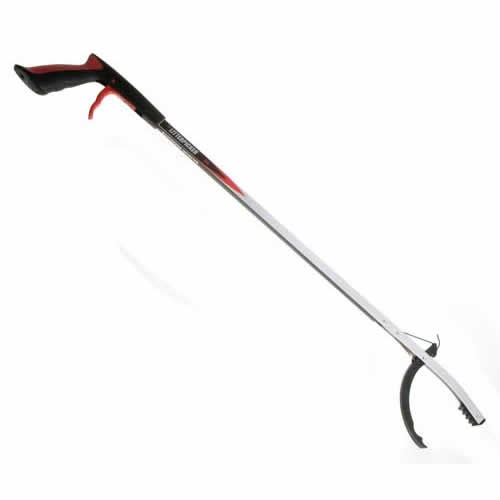
\includegraphics[width=0.5\textwidth]{Images/Gripper 6.png}
Eigenschaften: 
- sehr einfacher Aufbau
- wenige Teile notwendig
- nicht präzise Lösung

Greifer mittels 2 Zahnräder gleichmässig schliessen
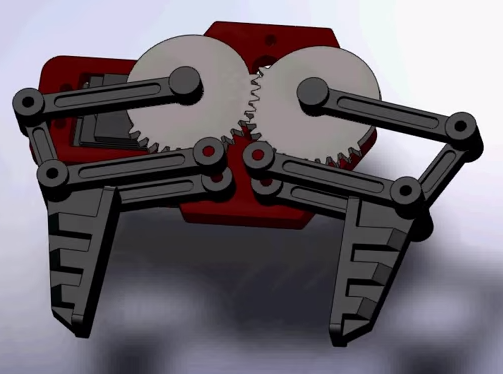
\includegraphics[width=0.5\textwidth]{Images/Gripper 2.png}
Eigenschaften:
- präzise Lösung
- aufwändiger Aufbau
- symmetrischer Aufbau

\subsection{pneumatisch}
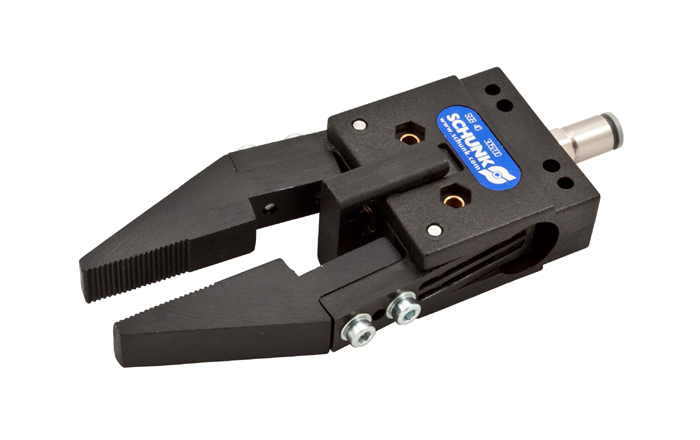
\includegraphics[width=0.5\textwidth]{Images/pneumatGr_schunk.jpg}
Eigenschaften: 
- Druckluft-Aggregat notwendig
- hohe Präzision
- teuer

\subsection{magnetisch}
Greifen der M4 Schrauben und Muttern mittels eines Elektromagneten
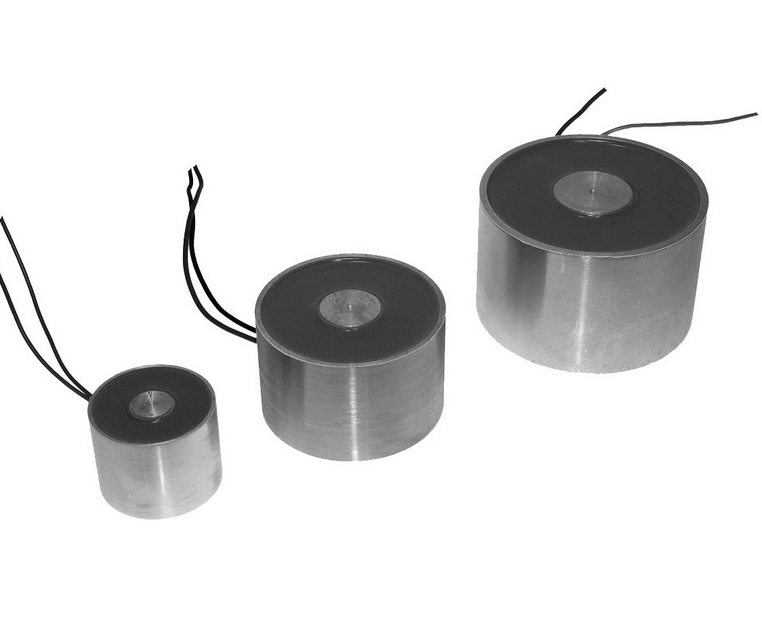
\includegraphics[width=0.5\textwidth]{Images/Magnetgreifer.png}
Eigenschaften:
- einfacher Aufbau
- einfache Integration
- fraglich ob genügend stark
